\section{User activity data on the Social Web} 
\label{sec:uad}
In order to answer the first research question, we have focused on data from two social services: \textit{YouTube} and
\textit{Twitter}. The goal of this chapter is to present the organization of the \textit{user activity data} (UAD)
available in those two networks.

In the section \ref{sec:youtube_uad} we describe user data available via APIs for
\textit{YouTube}, whereas section \ref{sec:twitter_uad} covers possible methods of extracting preference information
from \textit{Twitter} users' tweets. We will use the expression \textit{named entity} (NE) to refer to
known media people, shows and programs. The NE data has been collected from the \textit{Freebase} dataset,
which we described in section \ref{sec:vocabulary}.

\subsection{YouTube}
\label{sec:youtube_uad}

\textit{YouTube} stores various data concerning its users and content and offers a public
access to this structured information through the use of its API. In theory, additional
pieces of data could be acquired through the use of screen scraping. Using this
technique, however, breaks \textit{YouTube}'s Terms and Conditions (\S 5.1H), and as such
was not used for this research.

The schema of \textit{YouTube} data is presented in tables 1-5.  Each table lists
properties of a single type of entity, along with the way those properties are
accessed (either API or through the use of screen scraping). For example:
we can learn that values of such video's parameters as its view count or
its duration (and many others) are accessible through the official API.

Among these elements, what begs for most attention are the video sets.
Undoubtedly, videos are the central point of \textit{YouTube} as a service, and form the
majority of its content. This sets them as most suitable candidates for data
enrichment. Furthermore, the user can form a relation with a video by performing
an action on it (uploading, adding to favourites or subscribing), which makes
video analysis a perfect choice for semantic user profile generation.  Three
sets of videos are accessible through the official API, these are
\emph{favorites}, \emph{subscriptions} and \emph{uploads}. For this reason, the
rest of \textit{YouTube} research in this paper will focus on these three sets. The other
fields concerning user, like his \textit{age} or \textit{location}, while
directly usable as a part of the profile, are not as challenging to extract and
will not be analyzed in deep detail. \textit{YouTube} also contains demographic data
of a user, which we will not use in our experiments.

\begin{center}
  \begin{tabular}{|p{3cm} | l | p{4cm}|} \hline
  Information & Access & Notes\\ \hline
  Title & Public API & Natural language \\
  Published & Public API & \\
  Updated & Public API & Date \\
  Category & Public API & Chosen from a restricted set of YouTube categories \\
  Tags (keywords) & Public API & May be freely assigned \\
  Comments & Public API & Natural language \\
  Permissons & Public API & Irrelevant, but available \\
  Description & Public API & Natural language \\
  Thumbnails & Public API & Set of video's thumbnails (along with times
  when taken) \\
  Duration & Public API & \\
  Ratings & Public API & Best, worst and average rating, number of votes \\
  Viewcount & Public API & \\
  Favourite count & Public API & \\
  Number of likes & Public API & \\
  Number of dislikes & Public API & \\
  Aspect ratio & Public API & \\
  Related & Public API & \\
  Responses & Public API & \\
  Author & Public API & \\ \hline
  \end{tabular} \\
  Table 1: Information available for a video \\
\end{center}

\begin{table}[htb]
	\begin{minipage}[b]{0.5\linewidth}
	\centering
		\begin{tabular}{ | p{3cm} | l |}\hline
		Information & Access \\ \hline
		Number of results & Public API \\
		Search results & Public API \\ \hline
		\end{tabular}
		Table 2: Information available for video search results \\

		\begin{tabular}{ | p{3cm} | l |}\hline
			Information & Access \\ \hline
			Created & Public API \\
			Updated & Public API \\
			Author & Public API \\
			Text & Public API \\ \hline
		\end{tabular}
		Table 3: Information available for a comment \\

		\begin{tabular}{ | p{3cm} | l |}\hline
			Information & Access \\ \hline
			Demographics & Screen scraping \\
			Referrers & Screen scraping \\
			Countries popularity & Screen scraping \\ \hline
		\end{tabular}
		Table 4: Information available for a channel \\
	\end{minipage}
	\hspace{0.5cm} % no new lines here!!
	\begin{minipage}[b]{0.5\linewidth}
		\centering
		\begin{tabular}{ | p{3cm} | l |}\hline
			Information & Access\\ \hline
			\emph{Uploads} & Public API \\
			Gender & Public API \\
			Location & Public API \\
			Age & Public API \\
			Contacts & Public API \\
			Username & Public API \\
			\emph{Subscriptions} & Public API \\
			Inbox & Public API \\
			\emph{Favorites} & Public API \\
			History & Screen scraping \\
			Likes & Screen scraping \\
			Issued authentication subtokens & Screen scraping \\ \hline
		\end{tabular}
		Table 5: Information available for a user
		\label{ut_user_info}
	\end{minipage}
\end{table}

\subsubsection{Problems regarding concepts identification}

Even though the video sets are most promising mean to interest extraction. There
are problems that make this task challenging.

\paragraph{Detecting level of interest}
One of them, is the fact that YouTube videos cannot
express an interest directly. The user can add a video to the favourites
indicating some level of interest, but we are not able to detect the reason for
such user's action. This indirectness might result in lower precision of the
interests extracted from YouTube. 

The only indicator of an interest in a particular subject is binary: it is
either present or not present in user's data. This forces us to fall back to
entity counting in order to determine level of interest.

\paragraph{Usage of YouTube features} 
Another problem is the scarcity of data. Below are measurements that showed how
little users make extensive use of YouTube features.
In order to find out how frequently the mentioned sets are used, a sample of 7,500
randomly chosen users was examined. Among those users, noticeable differences in their
activity (level of use of various features) were noted. Many users show little activity,
as compared to a few highly active users.  50\% analyzed accounts had less than 60 favourites,
6000 out of 7,500 had less than 40 uploads.  All histograms on Figure 1 show
numbers of users (axis y) with $x_1-x_3$ numbers of
favourites/subscriptions/uploads. For all three cases, almost all users belonged
to the first histogram range -- the one with least items. As number of items
grows, the number of users decreases so quickly, that logarithmic scale has been
used in order to increase the readability of the charts.

For all three sets, almost half of examined users had no more than 100 items.
This means that for most cases, the user profiling would need to be based on
little amount of data.

\begin{figure}[htb]
  \centering
  \subfigure[Favourites]{
		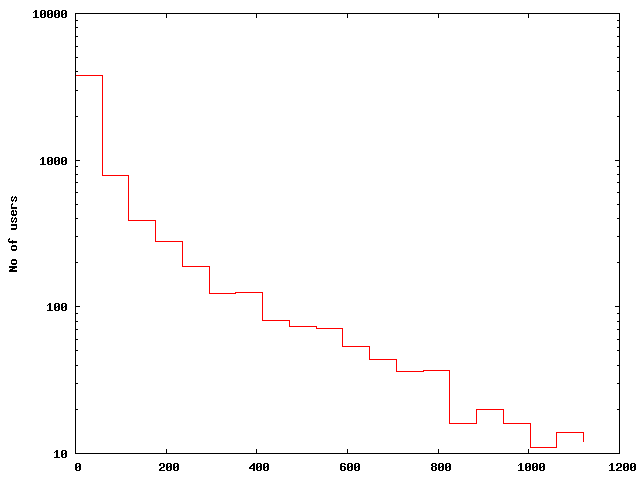
\includegraphics[scale=0.6]{images/favs.png}
		\label{fig:favs}
  }
  \subfigure[Subscriptions]{
		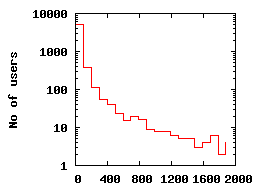
\includegraphics[scale=0.6]{images/subs.png}
		\label{fig:subs}
  }
  \subfigure[Uploads]{
		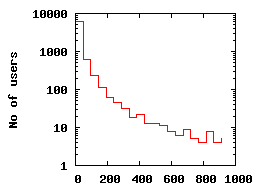
\includegraphics[scale=0.6]{images/ups.png}
		\label{fig:ups}
  }
  \label{fig:subfigureExample}
  \caption{Histograms of usage of favourites \subref{fig:favs}, subscriptions
  \subref{fig:subs} and uploads \subref{fig:ups}. The x axis represents groups of
  users having $x_1-x_2$ entities, the height of the bars indicates sizes of the
  groups.}
\end{figure}

\subsubsection{YouTube measurements employed}

We have decided to measure the user data in two ways: by identifying entities
and collecting tags. Each YouTube video contains a set of tags - single,
separate words - describing the video's content. While this kind of information
is not directly usable for the recommender systems, it can prove indirect
support for verifying the hypothesis that recommenders prepared. The types of
measurements performed are presented in Table 6.

\begin{center}
  \begin{tabular}{ | p{4cm} | p{7cm} | } \hline
    \multicolumn{2}{|c|}{Types of measurements available} \\
    \hline
    \multirow{3}{*} {Tag collection}
      & Tags from favourites \\ \cline{2-2}
      & Tags from subscriptions \\ \cline{2-2}
      & Tags from uploads \\ \cline{2-2}
    \hline
    \multirow{3}{*}{Concepts detection}
      & Concepts from favourites \\ \cline{2-2}
      & Concepts from subscriptions \\ \cline{2-2}
      & Concepts from uploads \\ \cline{2-2}
    \hline
  \end{tabular}
Table 6: Overview of the measures available for the \textit{YouTube} structured data \\
\end{center}

\subsubsection{YouTube video descriptions corpus}

A corpus of titles and descriptions for little over 100,000 videos was collected
for text-based analysis of YouTube data. The file's size was 36 Mbytes. This
data was used to compute number of video descriptions with identifiable concepts from
\textit{Freebase}\footnote{http://freebase.com} data vocabularies (more on this in section 4).

\subsection{Twitter}
\label{sec:twitter_uad}

Data available on \textit{Twitter} is composed of natural language short messages posted by users
consisting of up to 140 characters, commonly known as \textbf{tweets}. Within
those tweets we can distinguish user mentions (\textit{Twitter} usernames preceeded with the symbol @,
such as \textit{@justinbieber}\footnote{http://twitter.com/justinbieber}) as well as topics in form of
\textit{hashtags} -- names stripped of all whitespace and preceded by the hash symbol,
\eg \textit{\#TheDailyShow} \cite{edinburg-corpus}.

The initial purpose of tweets was to inform other users of currently performed activities. However, as this service has
evolved, users started to use \textit{tweets} for a variety of purposes, such as conversations,
sharing information/URLs and reporting news \cite{why-we-twitter, twitter-content-is-it}. In this section we describe available methods to use such unstructured data.
In our experiments we focus on the following NE extraction methods:

\paragraph{Mentioning NE full names}
Using simple string matching methods, we search for NE labels within tweets.
Occurrences of NE names in tweets indicate a potential interest in the NE mentioned. The
number of references is expected to be positively correlated with the level of interest in the given NE \cite{twitter-content-is-it}.
Entities might be mentioned by:
\begin{itemize}
  \item \textit{full name} (\eg \textit{"Having a How I Met Your Mother marathon."})
  \item \textit{hashtag} (\eg \textit{"Who?! Where? I love \#HowIMetYourMother!"})
  \item \textit{twitter username} (NE's twitter username, if known, \eg \textit{"@HIMYM\_CBS It entertains the spirit"})
  \item \textit{acronyms} (\eg \textit{"Watching HIMYM. Season 3."})
\end{itemize}
\paragraph{Usage of opinion vocabulary when tweeting about NEs}
In order to extract opinion towards a NE from a tweet, vocabularies that express
opinion has been compiled. They have been pragmatically chosen by looking at random tweets.
This vocabulary contains the following words: \textit{awesome, bad, enjoyed, good, great, hate,
like, liked, love, loving, poor, recommend, stunning, worst}.
Those verbs were searched for in the tweets containing NE mentions.
Example of a tweet: \textit{"yesterday's \#Lost episode was stunning!"}
\paragraph{Usage of activity verbs when tweeting about NEs}
When mentioning a media-related NE, users may also describe the activity performed.
In order to find such tweets, an activity verbs vocabulary has been prepared (similarly to
the opinion verbs, it was chosen by looking at the contents of random tweets).
This vocabulary contains the followings verbs: \textit{watching, watched, play,
watch, playing, saw, seen, played}.
Describing the activity of participating in a certain TV experience, such
as watching a show, has to be noted due to the fact that Twitter users are more
likely to specify what they are doing at a particular moment.
Example of a tweet: \textit{"Finnally watched Ironman 2 aha'"}

\paragraph{Extracting NEs from structured twitter stream sources}
Applications, such as \textit{YouTube} or \textit{Boxee}\footnote{http://www.boxee.tv}, automatically generate tweets
if the user linked their Twitter account with that application. These tweets are
usually well structured, and therefore very suitable to extract a NE, activity or preference.
Examples of tweets: (\textit{Boxee}) -- \textit{"likes Inglourious Basterds on Boxee http://bit.ly/FbAbn"} and
\textit{YouTube} -- \textit{"I liked a YouTube video -- How I Met Your Mother - Lorenzo Van Matterhorn"}

\paragraph{Summary}
We present the possible measurements for extracting the UAD from
\textit{Twitter} in Table 7:

\begin{center}
  \begin{tabular}{ | p{4cm} | p{7cm} | } \hline
    \multicolumn{2}{|c|}{Types of measurements available} \\
    \hline
    \multirow{4}{*} {Mentioning NEs}
      & Full name matching \\ \cline{2-2}
      & Matching the twitter username (if known) \\ \cline{2-2}
      & Matching name converted to a hashtag form \\ \cline{2-2}
      & Matching the full name acronym \\ \cline{2-2}
    \hline
    Usage of activity verbs & Mentions using activity verbs \\
    \hline
    \multirow{3}{*}{Using preference verbs}
      & Mentions using preference verbs \\ \cline{2-2}
      & Positive preferences \\ \cline{2-2}
      & Negative preferences \\ \cline{2-2}
    \hline
  \end{tabular}
Table 7: Overview of the measures available for the \textit{Twitter} UAD extraction \\
\end{center}

\subsubsection{Corpus used for research}

The example data analyzed consists of 43,000 tweets of 203 different users.
They have been selected by looking at the followers of popular TV channels and broadcasters
available on Twitter. Users were selected based on the number of tweets and their followers.
For our experiments, we have focused on tweets in English.

The most significant reason for using a precompiled corpus for this research is the Twitter API
Rate Limiting which limits the amount of tweets that can be fetched using the API.
Furthermore, a great deal of Twitter users provide data not necessarily
useful for our experiments. Mentions of NEs in non-English tweets could be located, but
extracting preference information in a multi-lingual setting is more challenging.
Using a preselected corpus enables measuring and comparing the effectiveness of different
counting methods much easier \cite{short-tweet}.

\subsection{Metrics used in constructing User Profile}

The generated user profile is a collection of concepts along with their
weights. In order to keep the scale of the weight simple (more on that in section
\ref{sec:evaluation}), we limited the scale to an integer range from 0
up to 3, meaning accordingly: ''do not like'', ''neutral'', ''like'', ''like
very much''. In order to determine the weight for each concepts, simple metrics
were used: number of repeats normalized to the mostly repeated item for
YouTube, and type of mention, the amount of mentions of a specified NE as well
activity/preference vocabulary usage for Twitter.

